\section{Results}
\label{sec:results}
\begin{table}[t]
\centering
\caption{Main policy comparison on \id/\ood evaluation. Best \ood robustness-calibration operating point is in \textbf{bold}.}
\label{tab:main}
\resizebox{\textwidth}{!}{%
\begin{tabular}{@{}lccccc@{}}
\toprule
\textbf{Policy} & \textbf{ID Acc} & \textbf{OOD Acc} & \textbf{Robustness Gap} & \textbf{Avg Tokens (OOD)} & \textbf{OOD ECE} \\
\midrule
\none & 1.000 & 0.367 & 0.633 & 212.0 & 0.2167 \\
\short & 1.000 & 0.700 & 0.300 & 234.1 & 0.2663 \\
\medium & 1.000 & 0.767 & 0.233 & 299.6 & 0.1947 \\
\longp & 1.000 & 0.700 & 0.300 & 381.4 & 0.2840 \\
\adaptive & 1.000 & \textbf{0.800} & \textbf{0.200} & 236.7 & \textbf{0.1823} \\
\bottomrule
\end{tabular}%
}
\end{table}


\para{Main finding: adaptive wins on \ood.}
\Tabref{tab:main} shows that all policies score 1.000 on \id, creating a ceiling effect. The important variation is therefore on \ood: \adaptive is best at 0.800, followed by \medium at 0.767. The no-trace policy drops to 0.367, confirming that minimal reasoning is brittle under shift. Robustness gap is smallest for \adaptive (0.200) and largest for \none (0.633).

\para{Non-monotonic fixed-length trend.}
Among fixed policies, \ood accuracy rises from \none $\rightarrow$ \short $\rightarrow$ \medium, then declines from \medium to \longp (0.767 to 0.700). This directional peak-and-drop pattern supports our non-monotonic hypothesis. A rank-based check over fixed policies yields Kendall $\tau=0.548$ ($p=0.279$), suggesting the trend but also limited power at current sample size.

\begin{table}[t]
\centering
\caption{Pairwise \ood comparison: \adaptive versus fixed policies. CI denotes paired bootstrap 95\% interval of accuracy difference.}
\label{tab:pairwise}
\resizebox{\textwidth}{!}{%
\begin{tabular}{@{}lcccc@{}}
\toprule
\textbf{Comparison} & \textbf{Acc Diff} & \textbf{95\% CI} & \textbf{McNemar $p$} & \textbf{BH $q$} \\
\midrule
\adaptive vs \none & +0.433 & [0.233, 0.633] & 0.0019 & 0.0078 \\
\adaptive vs \short & +0.100 & [-0.033, 0.267] & 0.3711 & 0.4948 \\
\adaptive vs \medium & +0.033 & [-0.100, 0.167] & 1.0000 & 1.0000 \\
\adaptive vs \longp & +0.100 & [-0.033, 0.267] & 0.3711 & 0.4948 \\
\bottomrule
\end{tabular}%
}
\end{table}


\para{Significance testing.}
\Tabref{tab:pairwise} shows a large and significant \adaptive improvement over \none (+0.433, BH-corrected $q=0.0078$). Differences against \short, \medium, and \longp are positive but not statistically significant, consistent with close performance among strong CoT policies at $N=30$ \ood items.

\begin{figure}[t]
    \centering
    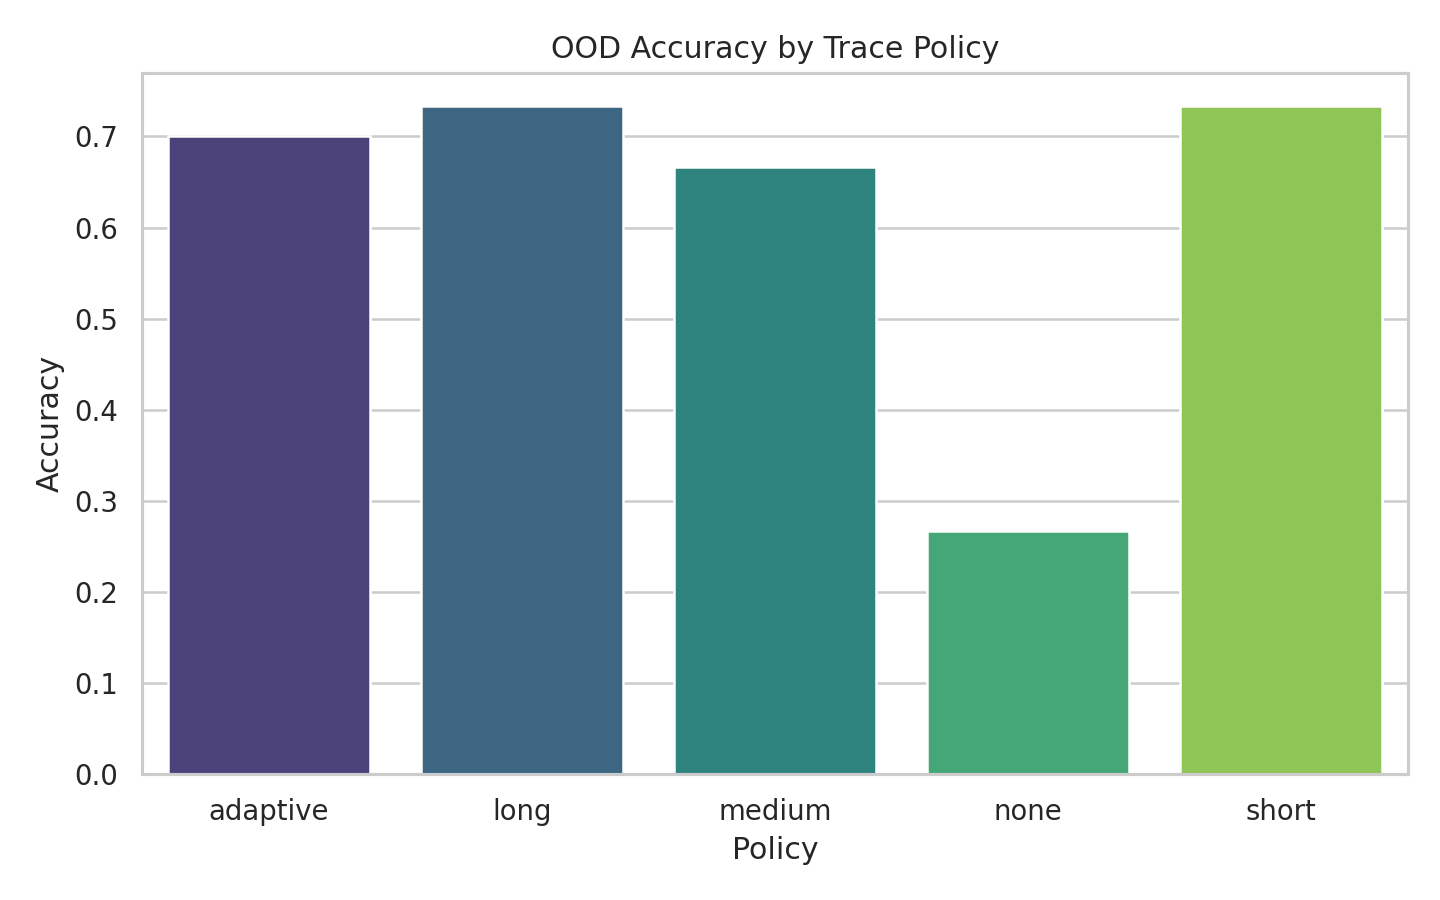
\includegraphics[width=0.95\linewidth]{../results/plots/ood_accuracy_by_policy.png}
    \caption{OOD accuracy by policy. The \adaptive policy reaches the highest value, while \none is substantially lower.}
    \label{fig:ood-acc}
\end{figure}

\begin{figure}[t]
    \centering
    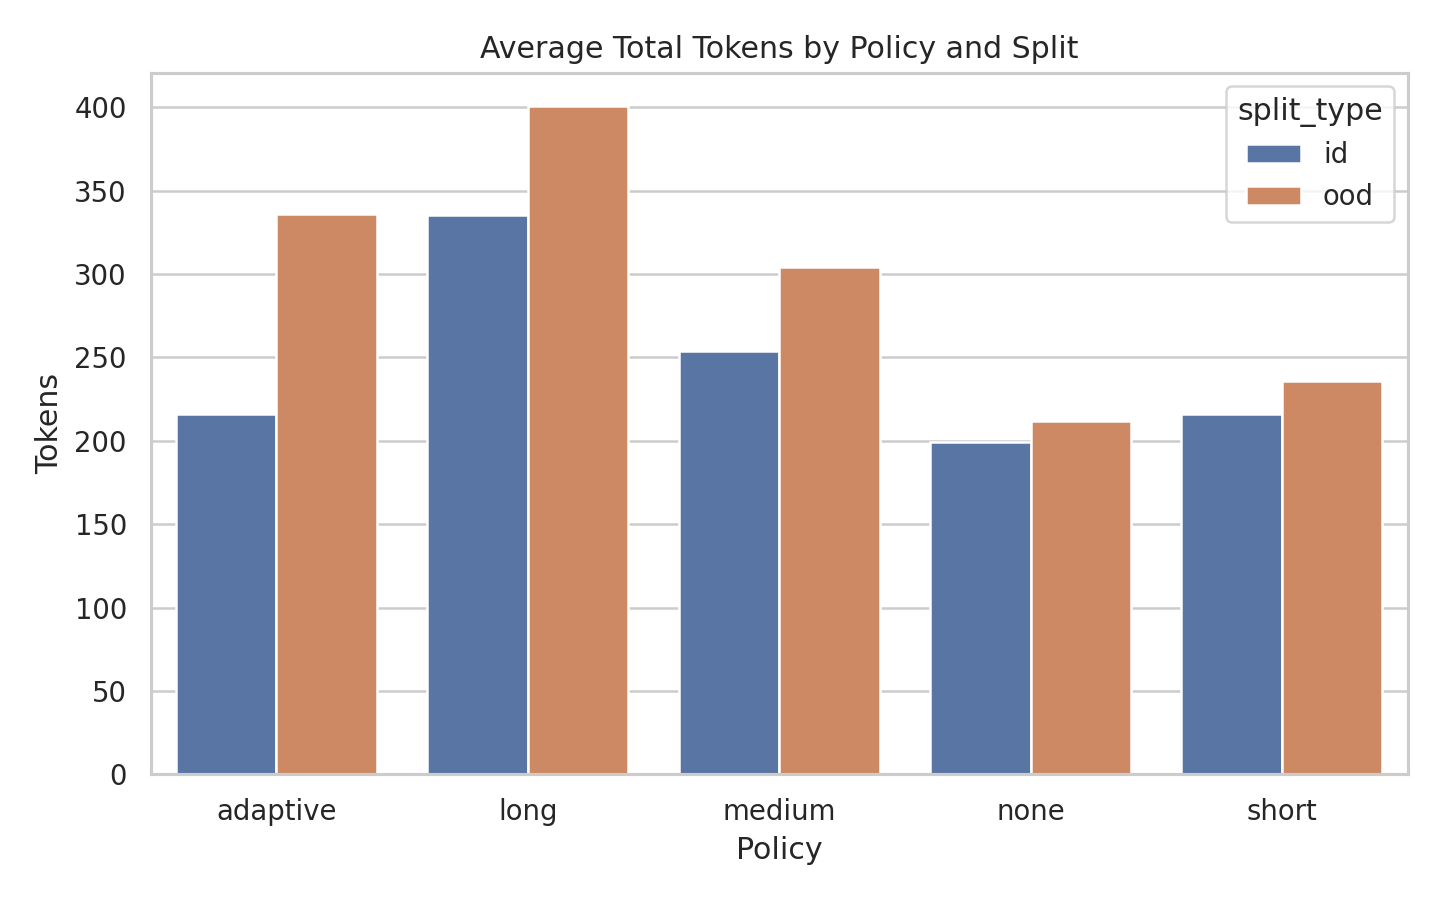
\includegraphics[width=0.95\linewidth]{../results/plots/token_usage_by_policy_split.png}
    \caption{Average token usage by split. \longp is the most expensive policy, while \adaptive remains close to \short and far below \longp.}
    \label{fig:tokens}
\end{figure}

\para{Calibration and efficiency.}
Despite high self-reported confidence across CoT-heavy modes, calibration differs meaningfully. \adaptive has the lowest \ood \ece (0.1823), while \longp has the worst (0.2840), indicating overconfident errors under very long traces. Token efficiency also favors \adaptive over \longp: similar or better \ood accuracy at much lower average token use (236.7 vs 381.4).

\para{Dataset-level behavior and errors.}
Performance is weakest on BBH date understanding and \mathfive. In \arc, \none fails completely on the sampled subset (0.000), while CoT-based policies recover strongly. Typical \adaptive failures include temporal-offset mistakes in date reasoning, option-format drift (letter vs phrase) in logical deduction, and strict-form mismatches for symbolic math outputs.
